
%(BEGIN_QUESTION)
% Copyright 2008, Tony R. Kuphaldt, released under the Creative Commons Attribution License (v 1.0)
% This means you may do almost anything with this work of mine, so long as you give me proper credit

Shown here is a view of a secant line and a tangent line (both thin) to a curve (thick):

$$\includegraphics[width=15.5cm]{i01508x01.eps}$$

The slope of one of these lines is represented by the ratio of two ``increments,'' $\Delta y$ and $\Delta x$:

$${\Delta y \over \Delta x}$$

\vskip 10pt

The slope of the other line is represented by the ratio of two ``differentials,'' $dy$ and $dx$, better known as a {\it derivative}:

$${dy \over dx}$$

\vskip 10pt

Determine which slope ($\Delta y \over \Delta x$ or $dy \over dx$) belongs to which type of line (secant or tangent), and label all increments and differentials on the graph.

\underbar{file i01508}
%(END_QUESTION)





%(BEGIN_ANSWER)

$$\includegraphics[width=15.5cm]{i01508x02.eps}$$

$${\Delta y \over \Delta x} = \hbox{ Slope of secant line}$$

\vskip 10pt

$${dy \over dx} = \hbox{ Slope of tangent line}$$

\vskip 10pt

Due to the classic definition of the derivative as being the limit of the secant line slope as $\Delta x$ approaches zero, many people are initially led to believe that $dx$ and $dy$ must necessarily be very small.  Not so!  Differentials such as $dx$ and $dy$ may assume any non-zero real number value, it's just that they indicate the slope of the tangent line, not the slope of the curve between intervals.  For practical applications of large-valued differentials, consult an introductory calculus book on the subject of {\it linear approximations} using differentials.

%(END_ANSWER)





%(BEGIN_NOTES)


%INDEX% Mathematics, calculus: derivatives and tangent lines
%INDEX% Mathematics, calculus: incremental ratios and secant lines

%(END_NOTES)


